\subsubsection{Mô tả thuật toán phát sinh khóa}

\noindent\textbf{2.1.1\quad Yêu cầu}
\begin{itemize}
    \item File cần crack: \texttt{WinCrackMe.exe}
    \item Công cụ sử dụng: \texttt{OllyDbg}
    \item File GENKEY cho chương trình: \texttt{crack2.exe}
\end{itemize}

\noindent\textbf{2.1.2\quad Hướng dẫn}
\begin{itemize}
    \item Khởi động chương trình bằng cách double-click vào file \texttt{WinCrackMe.exe}. Lúc này giao diện chương trình sẽ hiển thị như sau:
    \begin{figure}[H]
        \centering
        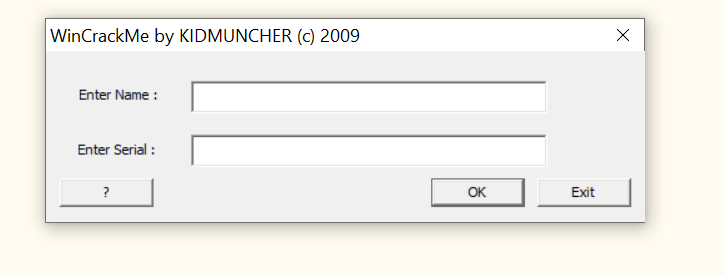
\includegraphics[width=\textwidth]{img/file-2/demo1.PNG}
        \caption{Giao diện chính của chương trình}
        \label{fig:main_interface}
    \end{figure}
    
    \item Chương trình hiển thị một hộp thoại chứa hai thuộc tính cần nhập vào (không bắt buộc): \texttt{Enter Name} và \texttt{Enter Serial}. 
    \item Bên trái dưới cùng là nút \texttt{'?'} hiển thị hướng dẫn, bên phải là nút \texttt{OK} và \texttt{Exit}.
    \begin{figure}[H]
        \centering
        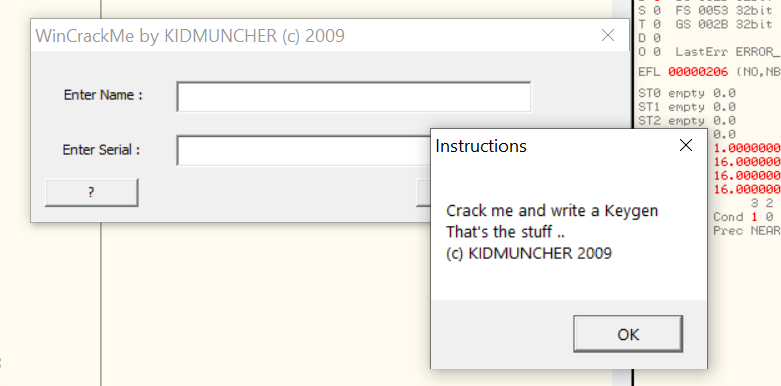
\includegraphics[width=\textwidth]{img/file-2/demo2.PNG}
        \caption{Hướng dẫn sử dụng chương trình}
    \end{figure}

    \item Các trường hợp có thể xảy ra:
    \begin{enumerate}[label=\textbf{TH\arabic*:}]
        \item Để trống cả hai thuộc tính:
        \begin{figure}[H]
            \centering
            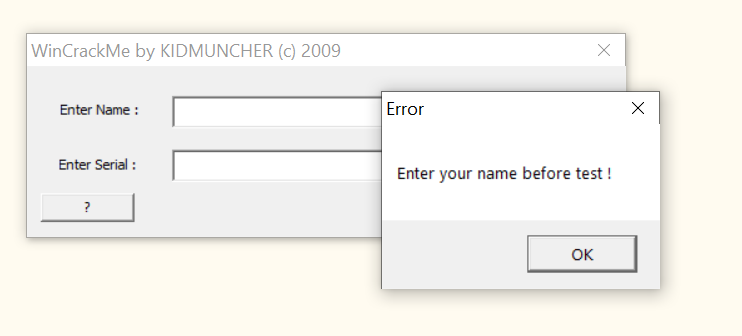
\includegraphics[width=0.8\textwidth]{img/file-2/demo3.PNG}
            \caption{Cả Name và Serial đều trống}
        \end{figure}
        
        \item Nhập \texttt{Name} với ít hơn 5 ký tự:
        \begin{figure}[H]
            \centering
            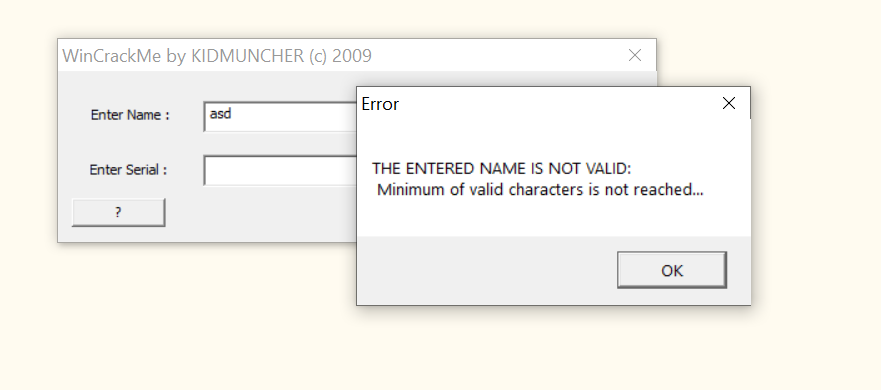
\includegraphics[width=0.8\textwidth]{img/file-2/demo4.PNG}
            \caption{Tên quá ngắn}
        \end{figure}
        
        \item Nhập \texttt{Name} chỉ gồm ký tự \texttt{a} hoặc \texttt{A}, đủ 5 ký tự:
        \begin{figure}[H]
            \centering
            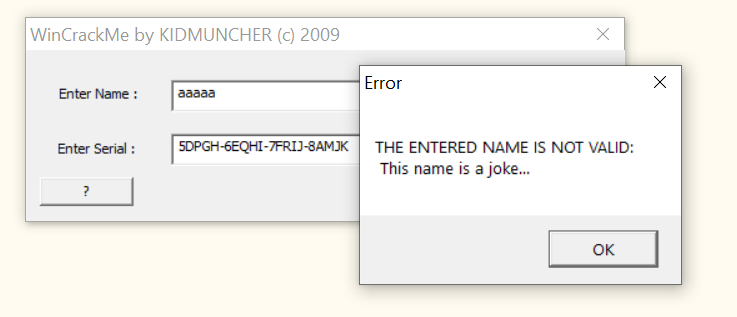
\includegraphics[width=0.8\textwidth]{img/file-2/demo5.PNG}
            \caption{Tên không đủ tốt}
        \end{figure}
        
        \item Nhập \texttt{Name} bất kỳ lớn hơn 5 ký tự:
        \begin{figure}[H]
            \centering
            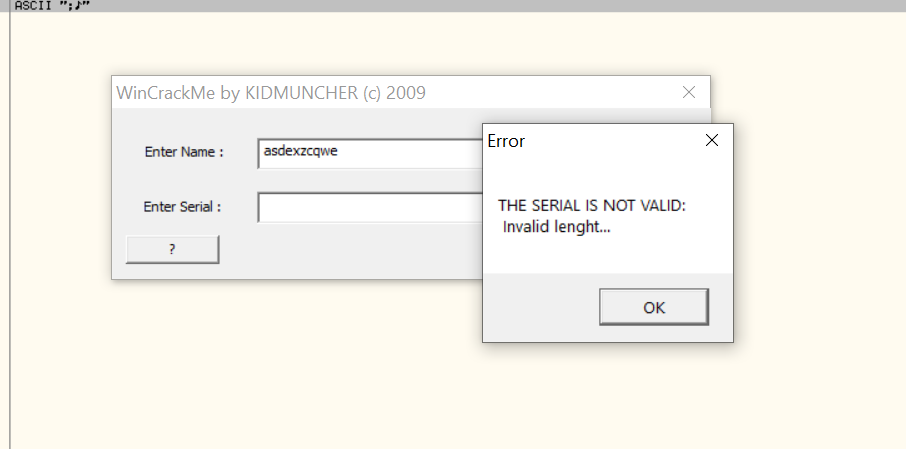
\includegraphics[width=0.8\textwidth]{img/file-2/demo6.PNG}
            \caption{Name hợp lệ nhưng Serial trống}
        \end{figure}
        
        \item Nhập \texttt{Serial} không đúng 23 ký tự:
        \begin{figure}[H]
            \centering
            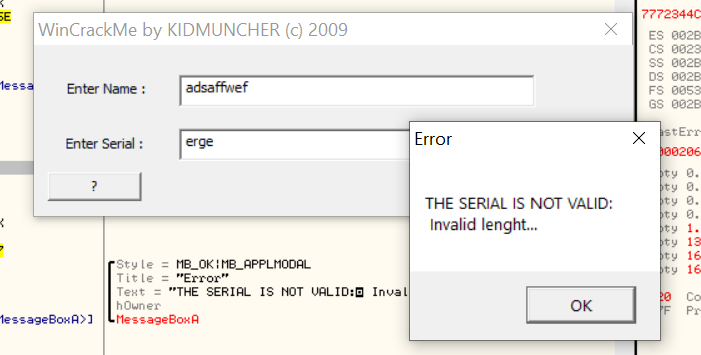
\includegraphics[width=0.8\textwidth]{img/file-2/demo9.PNG}
            \caption{Serial không đúng độ dài}
        \end{figure}
        
        \item Nhập \texttt{Serial} đúng 23 ký tự bất kỳ:
        \begin{figure}[H]
            \centering
            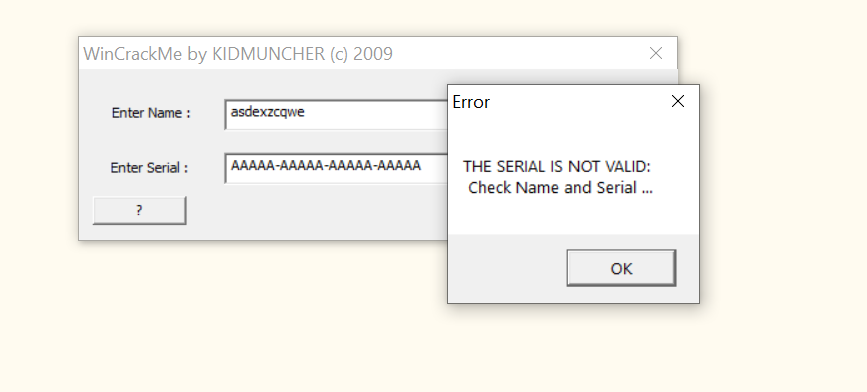
\includegraphics[width=0.8\textwidth]{img/file-2/demo7.PNG}
            \caption{Serial không hợp lệ}
        \end{figure}
        
        \item Nhập \texttt{Name} và \texttt{Serial} phù hợp:
        \begin{figure}[H]
            \centering
            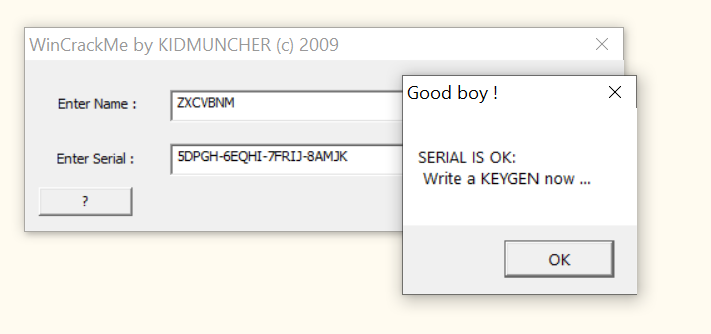
\includegraphics[width=0.8\textwidth]{img/file-2/demo8.PNG}
            \caption{Đăng nhập thành công}
        \end{figure}
    \end{enumerate}
\end{itemize}

\newpage
\noindent\textbf{2.1.3\quad Chi tiết phân tích chương trình}

\begin{itemize}
    \item Mở file \texttt{WinCrackMe.exe} bằng \texttt{OllyDbg}.
    \item Click chuột phải $\rightarrow$ \texttt{Search for > All referenced text strings}.
    \begin{figure}[H]
        \centering
        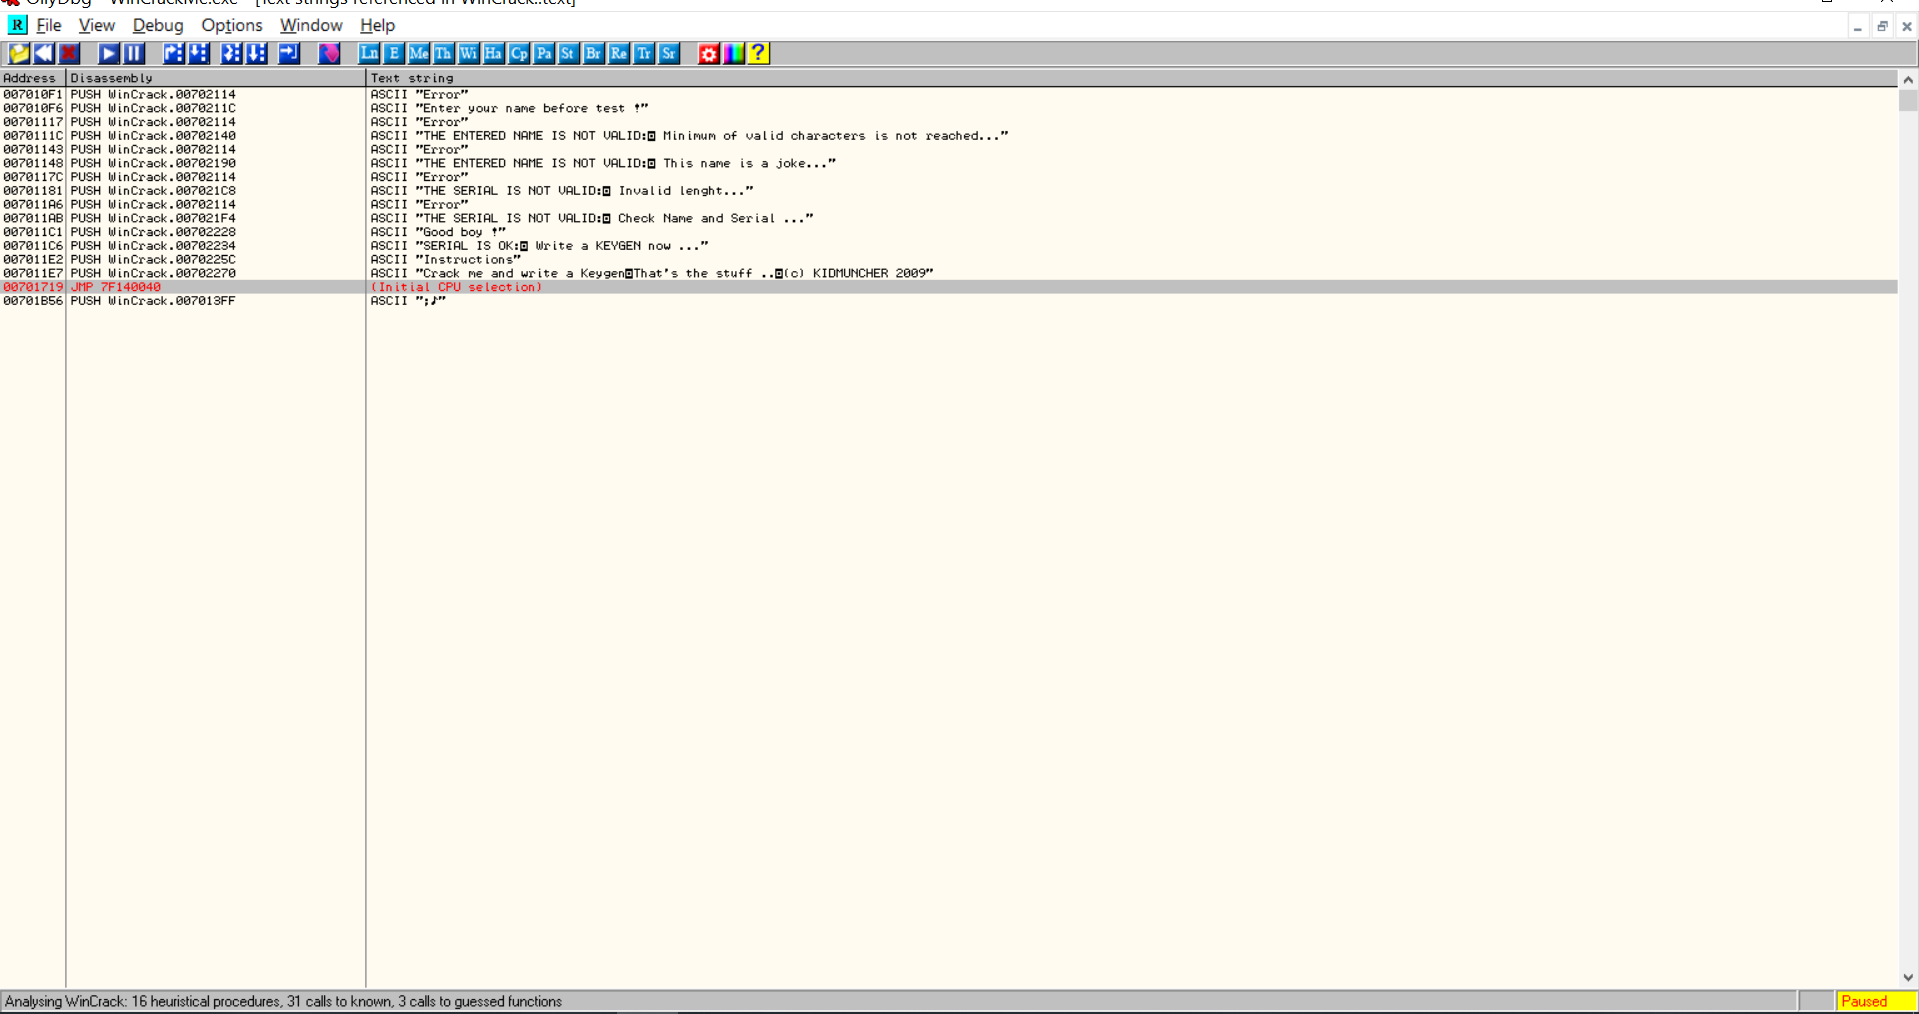
\includegraphics[width=\textwidth]{img/file-2/asm2.PNG}
        \caption{Danh sách chuỗi văn bản trong chương trình}
    \end{figure}
    
    \item Đặt Breakpoint tại đoạn code đầu tiên.
\end{itemize}

Các bước thực thi:
\begin{enumerate}[label=\textbf{Bước \arabic*:}]
    \item Nhập dữ liệu và nhấn \texttt{OK}. Chương trình dùng \texttt{GetDlgItemTextA} để lấy \texttt{Name} và \texttt{Serial}.
    \begin{center}
        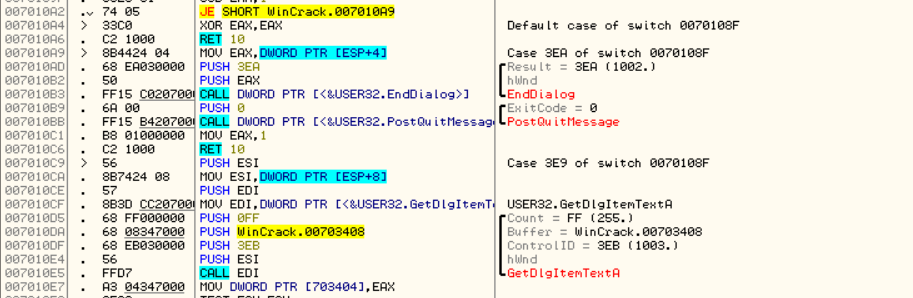
\includegraphics[width=0.8\textwidth]{img/file-2/asm3.PNG}
    \end{center}

    \item Kiểm tra \texttt{Name} có rỗng không với lệnh \texttt{TEST EAX, EAX}.
    \begin{center}
        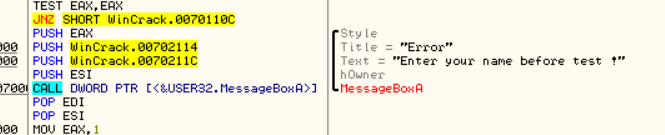
\includegraphics[width=0.8\textwidth]{img/file-2/asm4.PNG}
    \end{center}

    \item Kiểm tra số lượng ký tự chữ cái trong \texttt{Name} $\geq$ 5.
    \begin{center}
        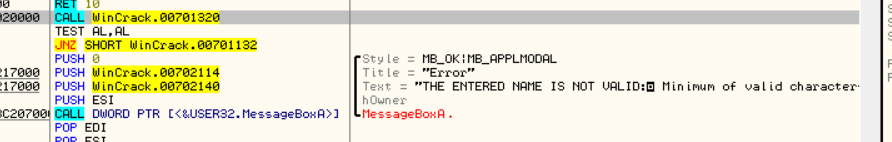
\includegraphics[width=0.8\textwidth]{img/file-2/asm5.PNG}
    \end{center}

    \item Tính giá trị \texttt{hash} từ \texttt{Name}.
    \begin{center}
        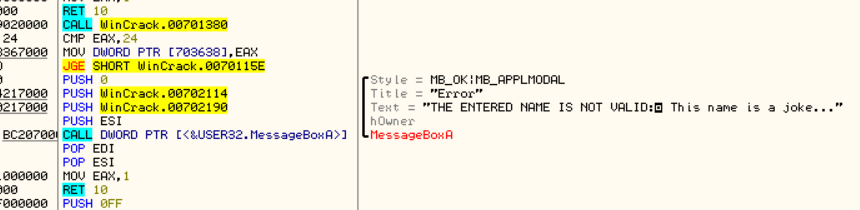
\includegraphics[width=0.8\textwidth]{img/file-2/asm6.PNG}
    \end{center}

    \item Kiểm tra độ dài \texttt{Serial} đúng bằng 23 ký tự.
    \begin{center}
        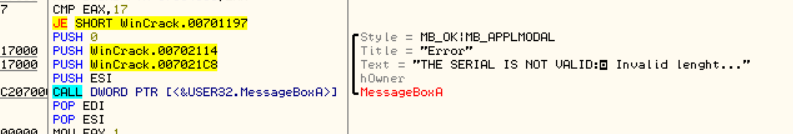
\includegraphics[width=0.8\textwidth]{img/file-2/asm7.PNG}
    \end{center}

    \item Tính \texttt{hash} từ \texttt{Serial} và so sánh với \texttt{hash} từ \texttt{Name}.
    \begin{center}
        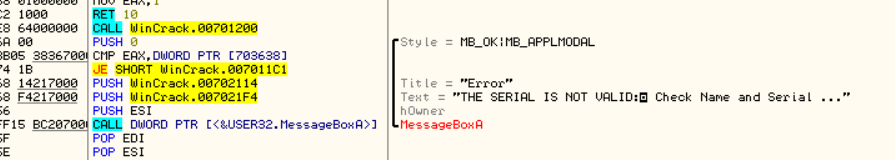
\includegraphics[width=0.8\textwidth]{img/file-2/asm8.PNG}
    \end{center}

    \item Nếu trùng khớp, hiển thị thông báo thành công.
    \begin{center}
        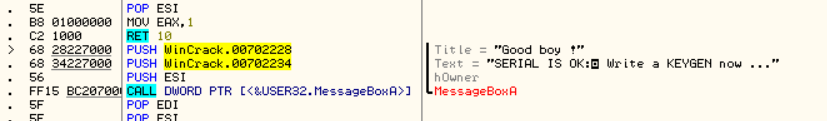
\includegraphics[width=0.8\textwidth]{img/file-2/asm9.PNG}
    \end{center}
\end{enumerate}

\subsubsection{Thuật toán phát sinh khóa}

\begin{itemize}
    \item \textbf{Tính hash của Name}:
        \begin{itemize}
        \item Hàm tính hash từ thuộc tính Name trong chương trình:
    \end{itemize}
        \begin{center}
        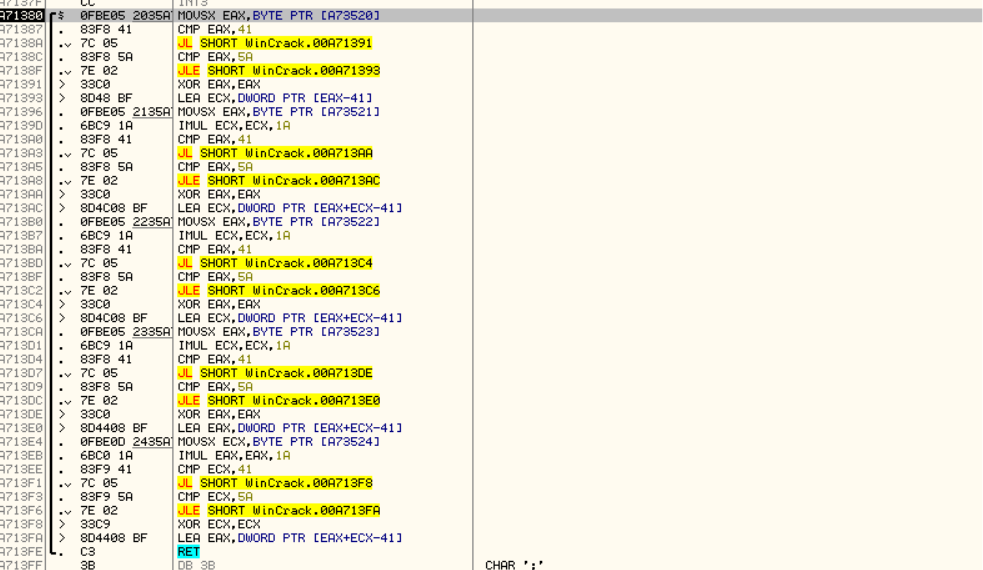
\includegraphics[width=0.8\textwidth]{img/file-2/asm11.PNG}
    \end{center}
    \begin{itemize}
        \item Chương trình sẽ kiểm tra các kí tự sao cho chúng là chữ cái in hoa hoặc in thường trong bảng ASCII. Các kí tự này đã được kiểm tra từ trước.
        \item Lấy 5 ký tự chữ cái đầu tiên, sau đó tính giá trị của nó dựa trên vị trí của chúng trong bảng chữ cái Alphabet. Lưu ý, các giá trị trong đoạn code trên dưới dạng HEX.
        \item Công thức tính giá trị hash như sau:
        \[
        hash = hash \times 1A + (\text{lower}(ch[i]) - 'a')(HEX)
        \]
        \[
        hash = hash \times 26 + (\text{lower}(ch[i]) - 'a')(DEC)
        \]
    \end{itemize}
    \begin{center}
        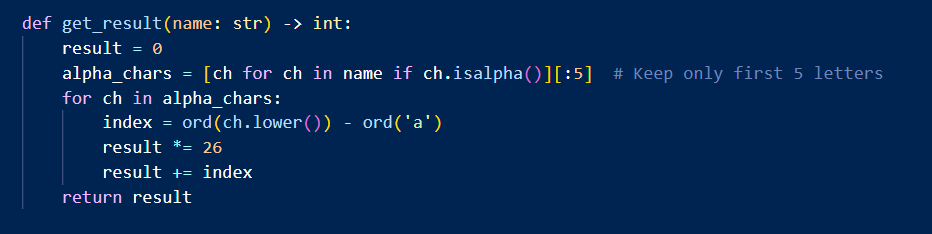
\includegraphics[width=0.8\textwidth]{img/file-2/code1.PNG}
    \end{center}
    
    \item \textbf{Tính hash của Serial}:
    \begin{itemize}
        \item Serial có 23 ký tự, chia thành 4 nhóm, mỗi nhóm 5 ký tự, ngăn cách bởi 1 dấu gạch ngang \texttt{-}.
        \item Sử dụng 4 bảng hash khác nhau ứng với từng nhóm, với mỗi bảng hash được rotate 1 đoạn cố định so với bảng hash trước.
        \item Công thức băm từng nhóm:
    \end{itemize}
    \begin{center}
        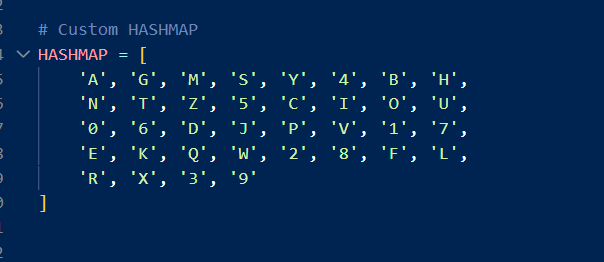
\includegraphics[width=0.8\textwidth]{img/file-2/code2.PNG}
        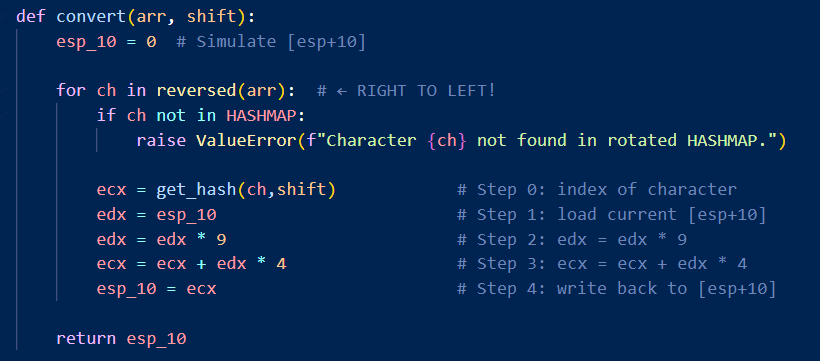
\includegraphics[width=0.8\textwidth]{img/file-2/code3.PNG}        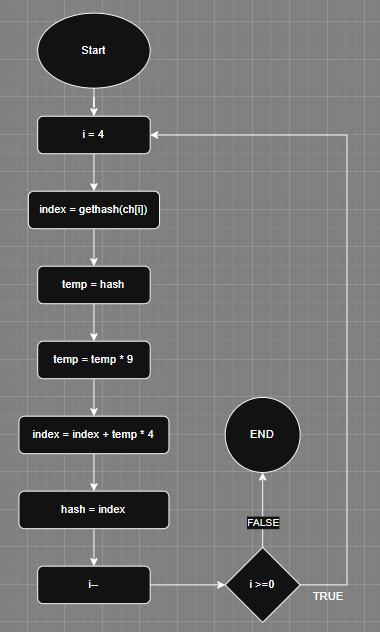
\includegraphics[width=0.8\textwidth]{img/file-2/img1.PNG}
    \end{center}

    \item \textbf{Điều kiện thành công}:
    \begin{itemize}
        \item Hash của tất cả 4 nhóm phải bằng nhau.
        \item Hash này phải trùng với hash của \texttt{Name}.
    \end{itemize}

    \item \textbf{Chương trình GENKEY}:
    \begin{itemize}
        \item Sử dụng thuật toán tham lam (\textit{Greedy Algorithm}) để tìm 1 giá trị Serial phù hợp với Name.
        \item Nhập Name vào chương trình GENKEY, Số Serial phù hợp được lưu vào file \texttt{key.txt}. 
    \end{itemize}
\end{itemize}

\newpage
\subsubsection{Kết luận}

Chương trình \texttt{WinCrackMe.exe} sử dụng kỹ thuật \textbf{hashing} để mã hóa và kiểm tra tính hợp lệ của dữ liệu đầu vào. Cụ thể:

\begin{itemize}
    \item Dữ liệu \texttt{Name} được xử lý bằng một hàm hash tuyến tính đơn giản, dựa trên 5 ký tự đầu tiên.
    \item Dữ liệu \texttt{Serial} được chia thành các nhóm, mỗi nhóm sử dụng một hàm băm phức tạp hơn với nhiều phép toán nhân, cộng và bảng ánh xạ riêng biệt, nhằm tạo ra tính ngẫu nhiên và tăng độ khó cho việc dò tìm bằng phương pháp brute-force.
    \item Cơ chế kiểm tra thành công dựa trên việc so khớp toàn bộ các giá trị hash đã tính từ \texttt{Name} và từng nhóm của \texttt{Serial}.
\end{itemize}

Việc phân tích mã assembly bằng công cụ \texttt{OllyDbg} giúp làm rõ luồng thực thi của chương trình và cách các hàm API Windows như \texttt{GetDlgItemTextA} được sử dụng để thu thập dữ liệu từ giao diện người dùng.

Bằng cách hiểu rõ thuật toán hashing nội tại, chúng tôi đã thiết kế được một chương trình \textbf{GENKEY} hoạt động hiệu quả, cho phép tự động sinh ra các cặp \texttt{Name} - \texttt{Serial} hợp lệ, đáp ứng mọi yêu cầu xác thực của ứng dụng.

\bigskip
\noindent\textbf{Ý nghĩa thực tiễn}:
\begin{itemize}
    \item Củng cố kỹ năng phân tích mã máy và dịch ngược (reverse engineering).
    \item Nâng cao kiến thức về kỹ thuật bảo mật phần mềm thông qua các thuật toán mã hóa nhẹ (lightweight hashing).
    \item Minh họa cách xây dựng công cụ hỗ trợ (GENKEY) dựa trên việc khai thác logic nội bộ của chương trình mục tiêu.
\end{itemize}

\bigskip
\noindent\textbf{Đánh giá tổng quát}: \\
Chương trình có mức độ bảo vệ cơ bản, chủ yếu dựa vào sự phức tạp của hàm băm hơn là cơ chế mã hóa mạnh mẽ. Với kiến thức về dịch ngược và phân tích thuật toán, việc xây dựng keygen phù hợp hoàn toàn khả thi.

\begin{lstlisting}
import sys

def get_result(name: str) -> int:
    result = 0
    alpha_chars = [ch for ch in name if ch.isalpha()][:5]  # Keep only first 5 letters
    for ch in alpha_chars:
        index = ord(ch.lower()) - ord('a')
        result *= 26
        result += index
    return result

def get_hash(ch: str, shift: int) -> int:
    # Find the original index of the character in the HASHMAP
    original_index = HASHMAP.index(ch)

    # Calculate the new index based on the shift (simulating rotation)
    rotated_index = (original_index - shift * 6) % len(HASHMAP)
    
    return rotated_index

# Get the hash key from the rotated HASHMAP
# based on the index and shift value
def get_hash_key(index: int, shift: int) -> str:
    # Get the character from the HASHMAP based on the index and shift
    rotated_index = (index + shift * 6) % len(HASHMAP)
    return HASHMAP[rotated_index]

def convert(arr, shift):
    esp_10 = 0  # Simulate [esp+10]
    
    for ch in reversed(arr):  # ← RIGHT TO LEFT!
        if ch not in HASHMAP:
            raise ValueError(f"Character {ch} not found in rotated HASHMAP.")

        ecx = get_hash(ch,shift)            # Step 0: index of character
        edx = esp_10                        # Step 1: load current [esp+10]
        edx = edx * 9                       # Step 2: edx = edx * 9
        ecx = ecx + edx * 4                 # Step 3: ecx = ecx + edx * 4
        esp_10 = ecx                        # Step 4: write back to [esp+10]

    return esp_10

# Custom HASHMAP
HASHMAP = [
    'A', 'G', 'M', 'S', 'Y', '4', 'B', 'H',
    'N', 'T', 'Z', '5', 'C', 'I', 'O', 'U',
    '0', '6', 'D', 'J', 'P', 'V', '1', '7',
    'E', 'K', 'Q', 'W', '2', '8', 'F', 'L',
    'R', 'X', '3', '9'
]



# Get serial 5 characters "XXXXX", default is "AAAAA"
def get_key_part(serial: str, index:int, shift:int, result: int) -> str:
    if (index == -1):
        return ''.join(serial)

    # Check if "XXXXX" hashvalue > result, ex: "AAAAA"
    # Save index of the indexed character
    for i in range(36):
        # Get first index+1 characters of the serial
        # and replace the indexed character with the current character
        text = list(serial)
        text[index] = get_hash_key(i, shift)
        
        temp = convert(text, shift)
        if temp > result:
            serial[index] = get_hash_key(i-1, shift)
            break
        elif temp == result:
            serial[index] = get_hash_key(i, shift)
            break
        
    # Recursion for remaning characters
    return get_key_part(serial, index-1, shift, result)

def get_key(result: int) -> str:
    serial = ['A' for i in range(23)]  # Start with "AAAAA"
    for i in range(3):
        serial[i*6+5] = '-'
        
    # Get the key part from the result
    for i in range(4):
        temp = [get_hash_key(0, i) for j in range(5)]  # Start with "AAAAA";
        temp = get_key_part(temp, 4, i, result)
        serial[i*6:i*6+5] = temp[:5]
    
    return ''.join(serial)

def save_key(name:str, key: str) -> None:
    with open("key.txt", "w") as f:
        f.write("Name: " + name + "\n")
        f.write("Serial code: " + key)

if __name__ == "__main__":
    name = input("Enter your name: ").upper()
    print("Your name is:", name)

    result = get_result(name)
    if result < 24:
        print("THE ENTERED NAME IS NOT VALID: This name is a joke...")
        exit(0)

    print("Converted value of name:", result)
    
    license_key = get_key(result)
    print("Found matching license key:", license_key)
    
    save_key(name, license_key)
    print("License key saved to key.txt")

\end{lstlisting}